\chapter{RESULTADOS}\label{chap:resultados}

Uma implementação do algoritmo EGSIS foi realizada como um projeto de
código-aberto e está disponível na plataforma
github\footnotemark. Nessa seção de resultados, avalia-se o
comportamento do método com variações no número de superpixels e
método de extração de características. Como referência para comparação
dos resultados, considera-se os métodos avaliados
em~\cite{wang2023review} no \textit{dataset} GrabCut.

\footnotetext{Disponível em \url{https://github.com/ryukinix/egsis/releases/tag/0.1.0}}

Uma avaliação qualitativa é demonstrada ao realizar a segmentação do
método e disponibilizar a máscara de segmentação gerada para algumas
imagens. Além disso, em formato de tabelas, é disponibilizada a
avaliação quantitativa baseada nas métricas descritos na
seção~\ref{sec:metricas-avaliacao}.

Por fim, foi desenvolvida uma ferramenta simples de anotação para
exploração dos resultados integrada ao software
JupyterLab\footnotemark, que é usada também para avaliação qualitativa
e visualização do impacto da anotação parcial inicial no resultado
final.

\footnotetext{Software web para desenvolvimento interativo e análise de dados, disponível em \url{https://jupyter.org}}

\section{Experimentos com a variação da quantidade de superpixels}\label{sec:variacao-superpixels}

Durante a execução dos experimentos, e avaliação dos resultados, foi
observado que o número de superpixels afeta diretamente a qualidade da
segmentação gerada. Entre esses experimentos, foram realizada 8
execuções com variações na técnica de extração de características
usada e no número de superpixels, sendo o número de superpixels
avaliados para 50, 100, 150 e 200.

\begin{table}[!h]
    \centering
    \Caption{\label{tab:variacao-superpixels} Resultados dos
experimentos ao variar o número de superpixels e o método de extração
de características. Em negrito os melhores resultados.}
  \begin{tabular}{lcccc}
    \toprule
    \textbf{Método}                  & \textbf{Recall} & \textbf{Precision} & \textbf{F1}     & \textbf{IoU}    \\
    \midrule \midrule
    $\gls{EGSIS}(s=50, f=gabor)$     & 0.7882          & 0.9225             & 0.8414          & 0.7412          \\
    $\gls{EGSIS}(s=100, f=gabor)$    & 0.8592          & 0.9505             & 0.8992          & 0.8232          \\
    $\gls{EGSIS}(s=150, f=gabor)$    & 0.8691          & 0.9550             & 0.9066          & 0.8354          \\
    $\gls{EGSIS}(s=200, f=gabor)$    & 0.8799          & \textbf{0.9620}    & 0.9167          & 0.8511          \\
    $\gls{EGSIS}(s=50, f=comatrix)$  & 0.7882          & 0.9225             & 0.8414          & 0.7412          \\
    $\gls{EGSIS}(s=100, f=comatrix)$ & 0.8617          & 0.9510             & 0.9010          & 0.8259          \\
    $\gls{EGSIS}(s=150, f=comatrix)$ & 0.8777          & 0.9552             & 0.9125          & 0.8441          \\
    $\gls{EGSIS}(s=200, f=comatrix)$ & \textbf{0.8877} & 0.9611             & \textbf{0.9212} & \textbf{0.8578} \\
    \bottomrule
  \end{tabular}
  \Fonte{\fonteautor}
\end{table}

Ao analisar a tabela~\ref{tab:variacao-superpixels}, é possível
perceber que o aumento de superpixels impacta positivamente na
qualidade da segmentação independente do método de extração de
características. A respeito do método de extração de características,
os resultados de ambos os métodos são próximos. Por outro lado, com
exceção da métrica de precisão, os melhores resultados vieram do
modelo com 200 superpixels e extração de características via matriz de
co-ocorrências.


\section{Avaliação qualitativa}

Nesta avaliação qualitativa, é comparada visualmente a qualidade
de segmentação do método \gls{EGSIS} com os melhores parâmetros
encontrados na seção anterior, isto é, número de superpixels definido
para 200 e método de extração de características via matriz de
co-ocorrências.

Como referência, o artigo~\cite{wang2023review} contém execuções
comparativas de vários métodos na base de dados GrabCut. Neste artigo,
é selecionado uma comparação com 16 imagens, nas quais 7 diferentes
métodos de segmentação interativa foram usados.

\begin{figure}[h!]
        \captionsetup{width=16cm}
		\Caption{\label{fig:grabcut-comparacao}
          Comparação entre diferentes métodos de segmentação interativa no dataset GrabCut.
        }
		\centering
		\UFCfig{}{\fbox{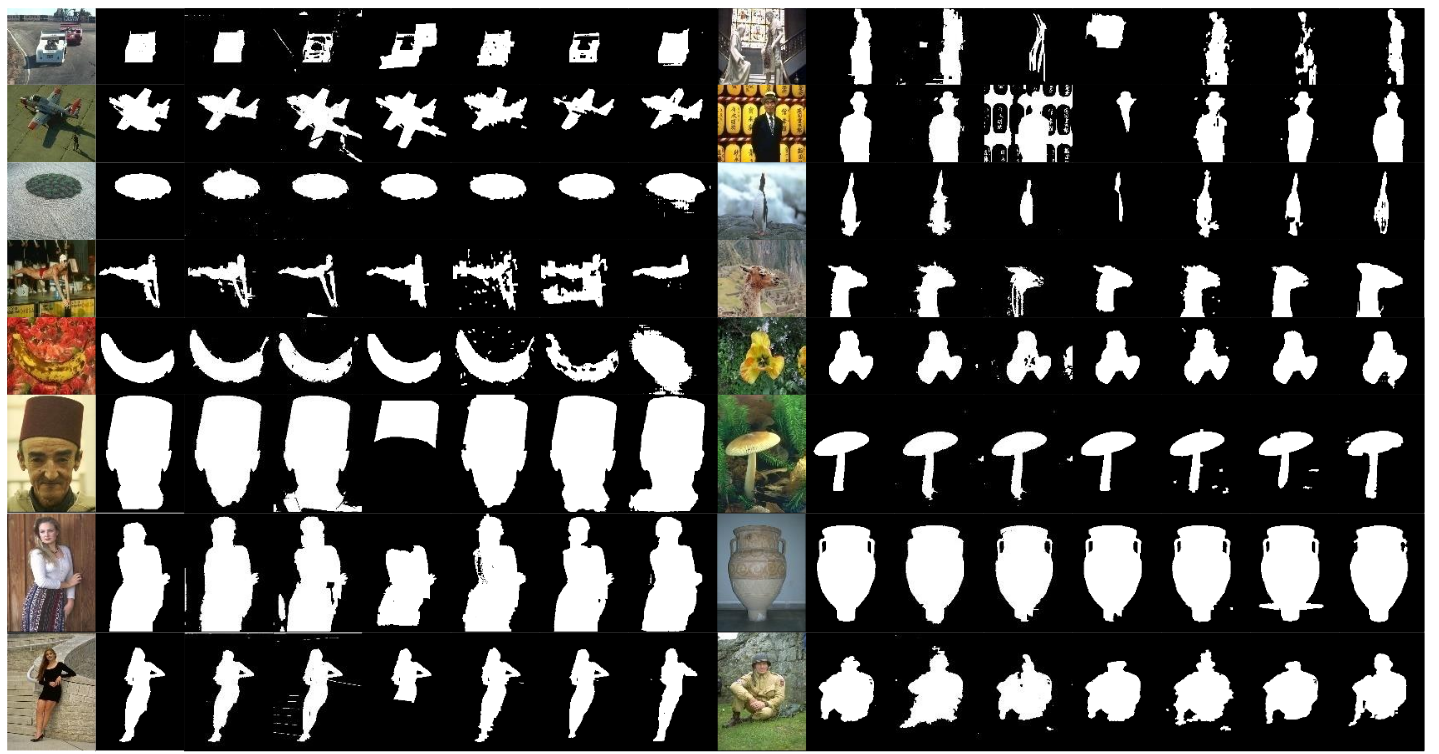
\includegraphics[width=16cm]{figuras/grabcut-comparacao}}}{\Fonte{\cite{wang2023review}}}
\end{figure}
\FloatBarrier{}

Na Figura~\ref{fig:grabcut-comparacao}, há em cada linha duas
imagems a ser segmentadas. Entre as máscaras de segmentação em escala
de cinza, há as segmentações dos métodos de segmentação
interativa. O nome desses 7 métodos, em ordem, são: GrabCut,
LazySnapping, OneCut, Saliency Cut, Iterated Graph Cuts, DenseCut e
Deep GrabCut.

Nesse aspecto, para comparação com o modelo proposto \gls{EGSIS}, para
as mesmas imagens do dataset GrabCut, são obtidas as seguintes máscaras
de segmentação na Figura~\ref{fig:egsis-qualitativa}.

\begin{figure}[h!]
        \captionsetup{width=12cm}
		\Caption{\label{fig:egsis-qualitativa}
          Execução de segmentação interativa com EGSIS, a primeira
segmentação é a do modelo e a última é a segmentação real.
        }
		\centering
		\UFCfig{}{\fbox{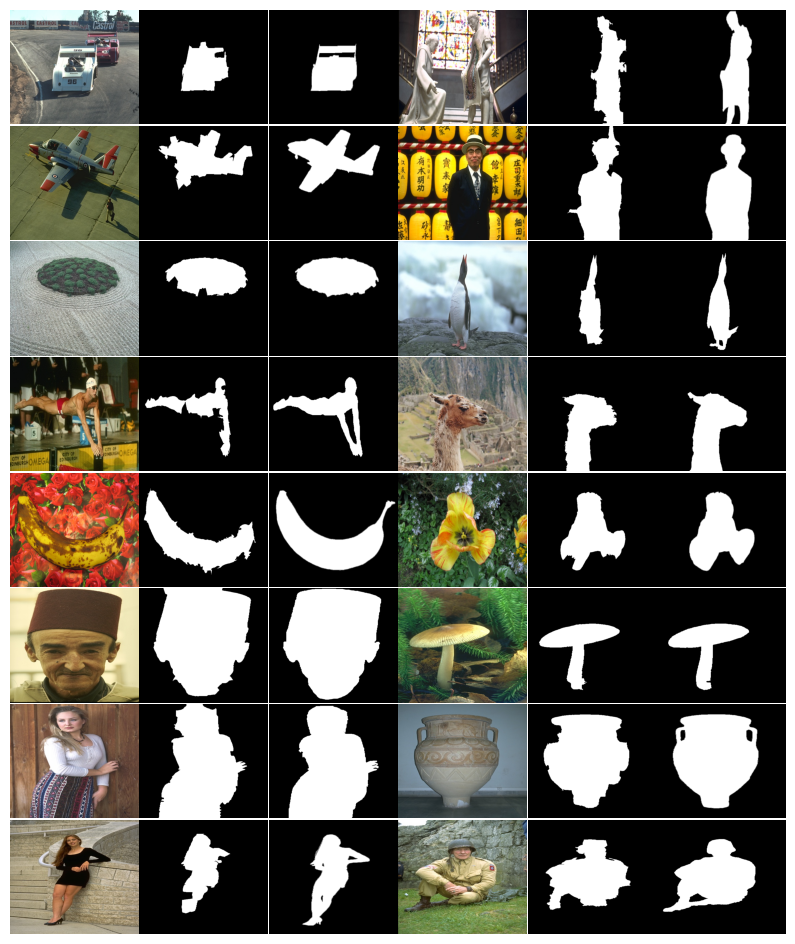
\includegraphics[width=12cm]{figuras/egsis-qualitativa}}}{\Fonte{\fonteautor}}
\end{figure}
\FloatBarrier{}



Como pode ser visto, os resultados do \gls{EGSIS} são de qualidade
comparável aos métodos comparados em~\cite{wang2023review}, embora em
algumas imagens haja mais erros e outras obtenham maior exito. Para
quantificar esse resultado, na próxima
seção~\ref{sec:comparacao-estado-da-arte} é realizada uma avaliação
quantitativa comparando esses métodos e o método proposto \gls{EGSIS}.


\section{Comparação quantitativa com o estado-da-arte da segmentação interativa}\label{sec:comparacao-estado-da-arte}

Nesta seção, é proposta uma avaliação de como o modelo \gls{EGSIS} se
compara ao estado-da-arte no problema de segmentação interativa.

No artigo~\cite{wang2023review}, é observado um extenso estudo de
revisão sobre os métodos de segmentação interativa baseados em grafos,
tendo como base o algoritmo GrabCut e outros algoritmos que evoluíram
nessa área de segmentação interativa de imagens. Os autores avaliam
essas técnicas na base de dados GrabCut~\cite{rother2004grabcut}
utilizando as mesmas métricas que foram selecionadas na metodologia de
avaliação deste trabalho, com exceção do tempo de execução, que, por
conta de diferentes tecnologias usadas para implementação das
técnicas, não foi possível usar para fazer uma avaliação justa, por
isso será deixada como um potencial trabalho futuro.

Esse mesmo artigo também avalia as várias técnicas em outro
\textit{dataset}, mas em virtude de a rotulação inicial usada não ter
sido publicada, não foi possível replicar os experimentos para o
modelo \gls{EGSIS} nas mesmas condições. Por esse motivo, a avaliação
de resultados será limitada a base de dados GrabCut.

A seguir, é possível visualizar tabelas de comparação com os
algoritmos apresentados em~\cite{wang2023review}: GrabCut,
LazySnapping, OneCut, Saliency Cut, Iterated Graph Cuts, DenseCut e
Deep GrabCut, todos algoritmos de segmentação interativa baseado em grafos.


\begin{table}[!h]
    \centering
    \Caption{\label{tab:resultados-estado-da-arte} Resultados
      comparativos entre o método EGSIS e métodos estado-da-arte para
      segmentação interativa baseado em grafos. Em negrito os melhores
      resultados.}
  \begin{tabular}{lcccc}
    \toprule
    \textbf{Método}                    & \textbf{Recall} & \textbf{Precision} & \textbf{F1}     & \textbf{IoU} \\
    \midrule \midrule
    GrabCut                            & 0.9668          & 0.9213             & \textbf{0.9407} & \textbf{0.8927}       \\
    LazySnapping                       & \textbf{0.9681} & 0.9104             & 0.9357          & 0.8842       \\
    OneCut                             & 0.8585          & 0.7926             & 0.7899          & 0.6974       \\
    Saliency Cuts                      & 0.8371          & 0.8892             & 0.8255          & 0.7458       \\
    Iterated Graph Cuts\footnotemark{} & 0.9614          & 0.8878             & 0.9212          & 0.8597       \\
    DenseCut                           & 0.8427          & 0.9418             & 0.8561          & 0.7927       \\
    Deep GrabCut                       & 0.8854          & 0.8774             & 0.8701          & 0.7849       \\
    $\gls{EGSIS}(s=200, f=gabor)$      & 0.8799          & \textbf{0.9620}    & 0.9167          & 0.8511       \\
    $\gls{EGSIS}(s=200, f=comatrix)$   & 0.8877          & 0.9611             & 0.9212          & 0.8578       \\
    \bottomrule
  \end{tabular}
  \Fonte{Baseado nos resultados encontrados no artigo~\cite{wang2023review}}
\end{table}

\footnotetext{Não há um nome formal pra esse método~\cite{an2013iterated}, por ora ele será chamado assim}
